Вернёмся к идее кросс-валидации:

\textit{Кросс-валидация} - это когда мы делим выборку на k кусочков, на k-1 используем как train, 1ый кусочек используем как валидацию. Потом берём второй кусочек, на остальных обучаемся и предсказываем на 2ом. И так проходимся по всем k кусочкам, то есть потребуется построить k моделей, тогда появится предсказание для каждого значения. В результате получается оценка эффективности выбранной модели с наиболее равномерным использованием имеющихся данных.

\begin{figure}[h]
\centering
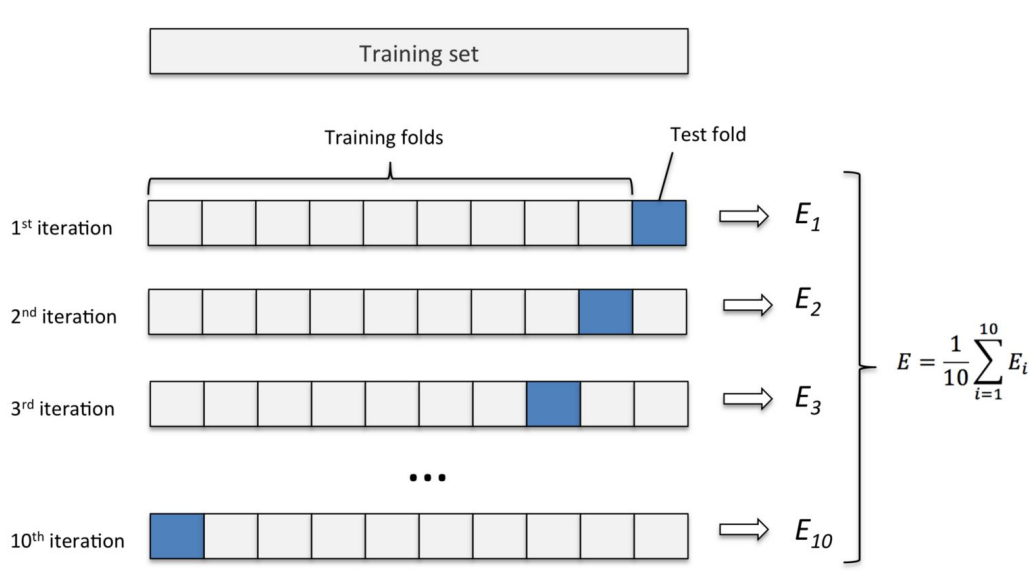
\includegraphics[width=0.5\linewidth]{14.1.PNG}
\caption{}
\end{figure}

Не путать кросс-валидацию и валидацию в целом.

Как соотносятся размеры тренировочной и валидационной выборки?(Вопрос из зала)

От 90/10 до 70/30, зависит от задачи и колиества данных. 

Note. Далее речь идет о K-fold кросс-валидации, где K — число запусков кросс-валидации и одновременно то, на сколько примерно равных кусков мы бьем train. 

Тогда в рамках каждого запуска один из K блоков является валидацией, а остальные — train.

Влияние количества блоков:

• При увеличении числа блоков дисперсия ответа уменьшается (закономерно, поскольку объем данных
увеличивается)

• Аналогичная ситуация с bias - матожидание разности между истинным ответом и выданным
алгоритмом - оно уменьшается.

• Чем меньше количество блоков, тем быстрее это работает, но тем меньше шанс, что модель
подстроится под какой-то кусок данных.

Кросс-валидацию следует делать, когда данных мало, потому что она работает лучше. Но, когда выборки огромные, делать кросс-валидацию очень долго. Используем Train, validation and test stage поскольку количество данных и так позволяет хорошо обучить модель.

\textit{Data leak} - утечка данных, при которой обучение происходит в том числе и на тестовых данных.
